\chapter{Descrição do problema}\label{cap:descprob}

%%%Aqui é a descrição do problema - Opcionalmente pode virar um capitulo.
  Os voos são organizados de forma que cada aeronave seja responsável por uma sequência válida, que é chamada de trilho.  O conjunto desses trilhos é a solução do problema e é denominada de malha. Essa malha deve conter o menor número possível de trilhos que atenda todos os voos planejados com o mínimo de modificações em relação ao planejamento inicial.
  
  As restrições que envolvem o PCTA induzem a formação de uma rede de possíveis conexões. Nessa rede os nós representam os voos e os arcos representam as conexões possíveis entre esses voos. Dessa forma o problema pode ser formulado como um problema de minimização de fluxos em uma rede.
  
  Dado a possibilidade de mudanças no tempo de partida sugerido dos voos e também a permissão para criar voos de reposicionamento, uma grande quantidade de soluções podem ser geradas. A ligação dos voos pode ocorrer de 6 formas distintas aqui denominado tipos de arcos. Os  arcos do tipo 1 permitem a ligação de voos sem a utilização de atrasos e/ou reposicionamento. Os arcos do tipo 2 utilizam atrasos mas não o reposicionamento. Os arcos do tipo 3 permitem o sequenciamento com a utilização de um voo de reposicionamento mas sem inserir atraso em nenhum dos voos envolvidos. Os arcos do tipo 4 utilizam-se de atrasos e de um voo de reposicionamento para fazer a ligação entre dois voos. Os arcos do tipo 5 e 6 são usados no modelo, que é baseado no fluxo em grafo, para representar respectivamente o nó origem(source) e o destino(sink). Abaixo um maior detalhamento desses arcos:

  
  \begin{itemize}
\item Conexão natural (Arco do tipo 1) - Os arcos desse tipo conectam dois voos respeitando o tempo de partida sugerido e
a restrição geográfica. Eles são associados com as ligações que não requerem mudanças no tempo de partida e nem
       precisam de voos de reposicionamento. O arco do tipo 1 não apresenta custo para ser adicionado a solução.

\begin{figure}[ht]
	\centering
	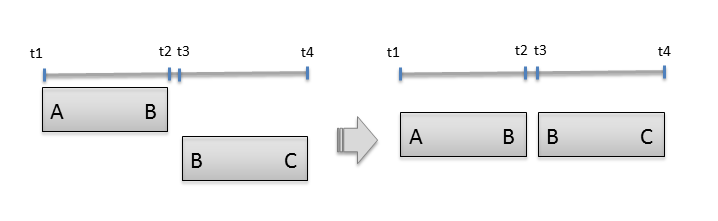
\includegraphics[scale=0.35]{./img/arc1}
	\caption{Representação esquemática do arco do tipo 1}
	\label{fig:arc1}
\end{figure}

\item Mudança no tempo (Arco do tipo 2) - Apesar de ter os voos incidentes no mesmo aeroporto, os arcos desse tipo não
permitem a ligação de forma direta pois o tempo de solo disponível não é suficiente para permitir a ligação. No
      entanto, a escolha desse tipo de arco implica em uma mudança no tempo de partida sugerido para quaisquer um dos
      voos envolvidos. O custo de um arco desse tipo é igual a soma dos valores absolutos dos atrasos (em minutos) dos
      horários de partida envolvidos.
      
\begin{figure}[ht]
	\centering
	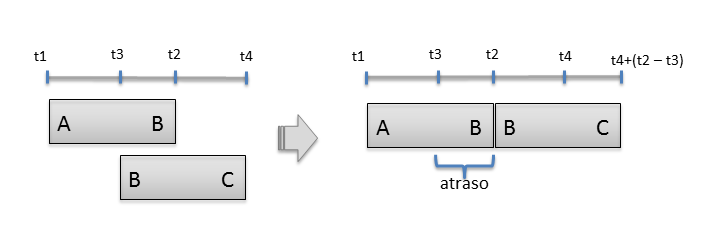
\includegraphics[scale=0.35]{./img/arc2}
	\caption{Representação esquemática do arco do tipo 2}
	\label{fig:arc2}
\end{figure}

\item Voos de reposicionamento (Arco do tipo 3) - Esses arcos representam conexões entre dois voos em que a origem
parte de um aeroporto diferente do local de partida do voo de destino, no entanto, existe tempo suficiente para um voo
de reposicionamento, entre os dois locais, sem violar as restrições de tempo de solo. Os custos de um arco do tipo 3 é
  igual a duração do voo de reposicionamento, incluindo o seu tempo de solo.

\begin{figure}[ht]
	\centering
	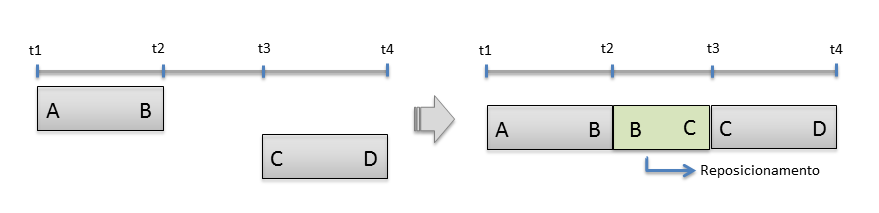
\includegraphics[scale=0.35]{./img/arc3}
	\caption{Representação esquemática do arco do tipo 3}
	\label{fig:arc3}
\end{figure}

\item Voos de reposicionamento mais mudança de tempo (Arco do tipo 4) - Esses arcos representam conexões que
precisam de um voo de reposicionamento mais mudança no tempo de partida sugerido. O arco do tipo 4 tem custo
igual tempo do voo de reposicionamento, incluindo o tempo de solo, mais a soma dos atrasos dos horários de partida
envolvidos em valor absoluto.

\begin{figure}[ht]
	\centering
	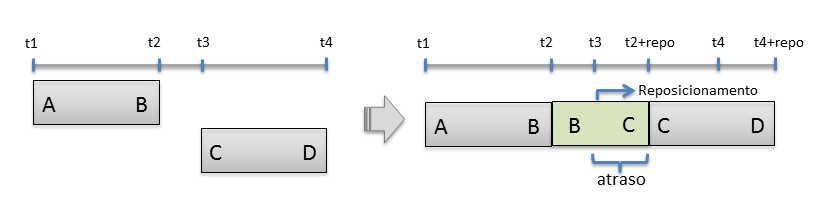
\includegraphics[scale=0.35]{./img/arc4}
	\caption{Representação esquemática do arco do tipo 4}
	\label{fig:arc4}
\end{figure}

\item Arcos do nó fonte ou \textit{source} (Arco do tipo 5) - Esses, arcos são criados para identificar o inicio de um trilho e é com
 ele também que se sabe a quantidade de trilhos necessários para resolver o problema. Cada arco do tipo 5 tem o custo
  igual a 1000.

\item Arcos do nó final ou \textit{sink} (Arco do tipo 6) - Esses arcos tem como destino o nó fictício que é usado para finalizar um
  trilho no modelo. Os arcos do tipo 6 não tem custo.

\end{itemize}

Abaixo na Figura \ref{fig:arpexample} temos dois exemplos de montagem de trilhos feitas a partir de um conjunto fictícios de voos. Cada caixinha laranja e azul representa um voo, onde a parte laranja representa o tempo de solo que cada voo deve obedecer e a azul seria o tempo de voo da cidade de origem para a cidade de destino. As letras A, B, C, D, E representam as cidades e a linha pontilhada indica o tempo de inicio e de termino de cada voo.

\begin{figure}[ht]
	\centering
	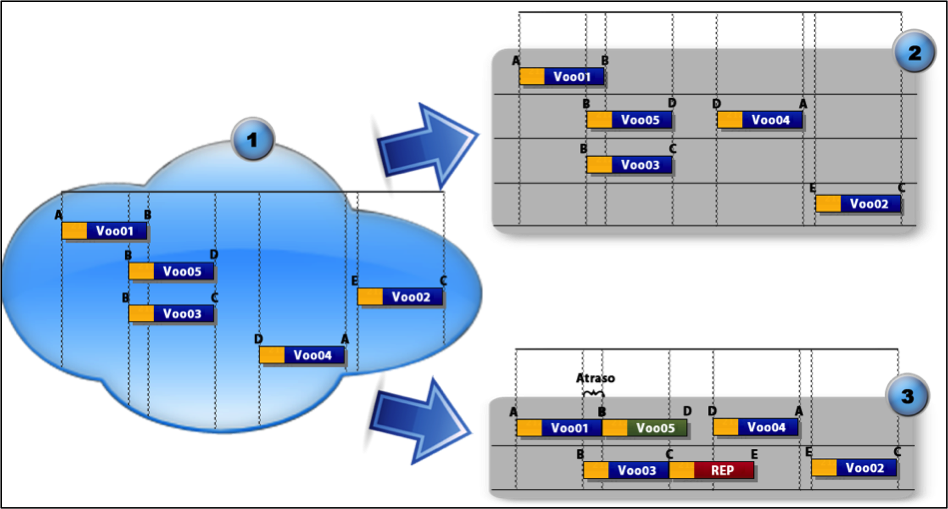
\includegraphics[scale=0.9]{./img/arpexample}
	\caption{Construção de Trilhos de Aeronaves}
	\label{fig:arpexample}
\end{figure}

A parte 1 da Figura \ref{fig:arpexample} representa os voos da companhia que ainda não foram cobertos por nenhuma aeronave e nas partes 2 e 3 são demonstrado duas formas de organizar esses voos em trilhos. 

	Na parte 2 temos a melhor forma possível de se organizar os voos da parte 1 utilizando apenas os arcos do tipo 1, ou seja sem a utilização de atrasos ou de voos de reposicionamento. Dessa forma se consegue uma formação com 4 trilhos.

	Na parte 3 temos a melhor forma de organizar os voos utilizando todos os arcos e um atraso máximo equivalente a um tempo de solo. Dessa forma se consegue uma formação com apenas 2 trilhos.

	Pode-se verificar que a utilização de diferentes tipos de arcos pode proporcionar uma melhora significativa  no número de trilhos. Porém essa abordagem faz com que o número de soluções possíveis tenha uma cardinalidade muito superior a utilização de arcos apenas do tipo 1 que por si só já gera uma quantidade de soluções bem elevada, por isso os arcos devem ser utilizados de forma controlada. 


  
%%%% Até aqui %%%%%%%%%%